\section{Цель работы}
Целью данной работы является изучение метода Гаусса-Зейделя решения
систем линейный алгебраических уравнений.

\section{Описание метода}
Метод Гаусса-Зейделя --- итерационный метод решения систем линейных алгебраических
уравнений.
Ключевым отличие метода Гаусса-Зейделя от метода простых итераций является
использование компонент \(x_1^{(k+1)}, x_2^{(k+2)}, \ldots, x_{i-1}^{(k+1)}\)
при вычислении компоненты \(x_i^{(k+1)}\).
За счет этого метод обеспечивает более быструю сходимость.

Основной рабочей формулой метода Гаусса-Зейделя является формула
\begin{equation}
	x_{i}^{(k+1)} = \frac{b_i}{a_{i,i}} - \sum_{j = 1}^{i-1} \frac{a_{i,j}}{a_{i,i}} x_j^{(k+1)} -
	\sum_{j=i+1}^{n} \frac{a_{i,j}}{a_{i,i}} x_{j}^{(k)}
	\label{eq:gauss_seidel:1}
\end{equation}

Формулу (\ref{eq:gauss_seidel:1}) можно преобразовать к использованию матрицы \(C\) и вектора \(d\) таких, что
\[ x = Cx + d \]
\[
	c_{i,j} = \begin{cases}
		0,                         & i = j    \\
		- \frac{a_{i,j}}{a_{i,i}}, & i \neq j
	\end{cases}
	\qquad
	d_i = \frac{b_i}{a_{i,i}}
\]

Таким образом, получаем формулу:
\begin{equation}
	x_{i}^{(k+1)} = \sum_{j=1}^{i-1} c_{i,j} x_j^{(k+1)}
	+ \sum_{j=i+1}^{n} c_{i,j} x_j^{(k)} + d_1
	\label{eq:gauss_seidel:2}
\end{equation}

\section{Листинг программы}
\inputminted[breaklines]{Rust}{./src/solution.rs}

\section{Примеры и результаты работы программы}
На рис.~\ref{fig:example:1} представлен пример работы программы для СЛАУ.
Входные данные вводятся с файла.
\begin{equation}
	\begin{cases}
		2 x_1 + 10 x_2 + x_3   & = 13 \\
		10 x_1 + x_2 + x_3     & = 12 \\
		2 x_1 + 2 x_2 + 10 x_3 & = 14
	\end{cases}
	\label{eq:sample:1}
\end{equation}
\begin{figure}[H]
	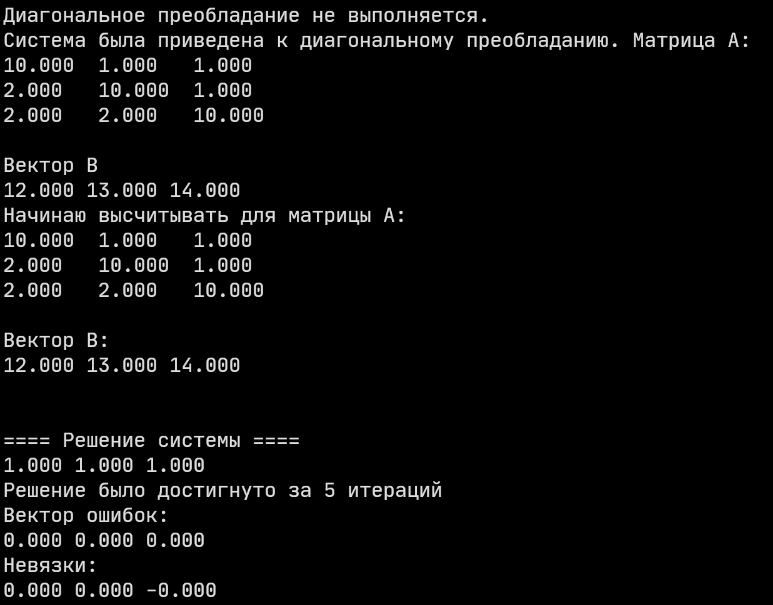
\includegraphics[width=\textwidth]{./img/test1.png}
	\caption{Работа программы для СЛАУ~(\ref{eq:sample:1}) и точности \(\varepsilon = 10^{-4}\)}
	\label{fig:example:1}
\end{figure}

На рис.~\ref{fig:example:2} представлен пример работы для матрицы, которую нельзя привести к
диагональному виду.
\begin{figure}[H]
	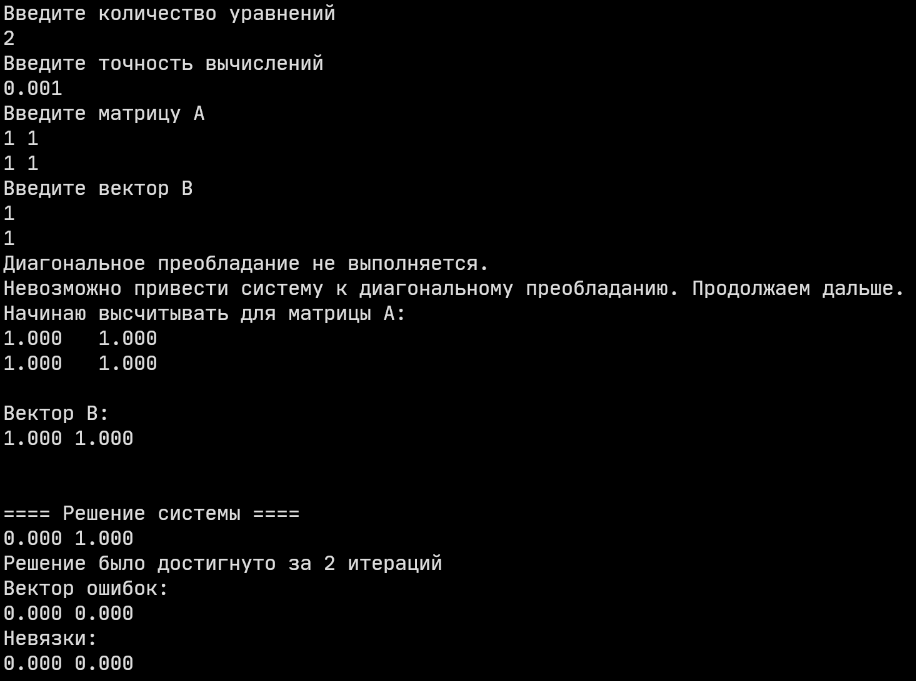
\includegraphics[width=\textwidth]{./img/test2.png}
	\caption{Работа программы для СЛАУ, которую нельзя привести к диагональному виду}
	\label{fig:example:2}
\end{figure}

На рис.~\ref{fig:example:3} представлен пример работы для СЛАУ, соответствующего матрице \(A\) и вектору \(b\), заданным в (\ref{eq:example:3}).
\begin{equation}
	A = \begin{pmatrix}
		100   & 1 & 2   & 3   & 4   & 5   & 6   & 7   & 8   & 9    \\
		1 200 & 2 & 3   & 4   & 5   & 6   & 7   & 8   & 9          \\
		1     & 1 & 300 & 3   & 4   & 5   & 6   & 70  & 8   & 9    \\
		1     & 1 & 2   & 400 & 4   & 50  & 6   & 7   & 8   & 9    \\
		1     & 1 & 2   & 3   & 500 & 5   & 6   & 7   & 8   & 9    \\
		1     & 1 & 2   & 3   & 4   & 5   & 60  & 7   & 8   & 1000 \\
		1     & 1 & 2   & 3   & 4   & 600 & 6   & 7   & 8   & 9    \\
		1     & 1 & 2   & 3   & 4   & 5   & 700 & 7   & 8   & 9    \\
		1     & 1 & 2   & 3   & 4   & 5   & 6   & 800 & 700 & 9    \\
		1     & 1 & 2   & 3   & 4   & 5   & 6   & 7   & 900 & 9    \\
	\end{pmatrix}
	\quad
	B = \begin{pmatrix}
		141234.123     \\
		1123.3213      \\
		-11234123.321  \\
		-234132.645654 \\
		12314.123123   \\
		-112.3123656   \\
		11242135.1323  \\
		-123423.3123   \\
		112384.12374   \\
		1307.37637
	\end{pmatrix}
	\label{eq:example:3}
\end{equation}

\begin{figure}[H]
	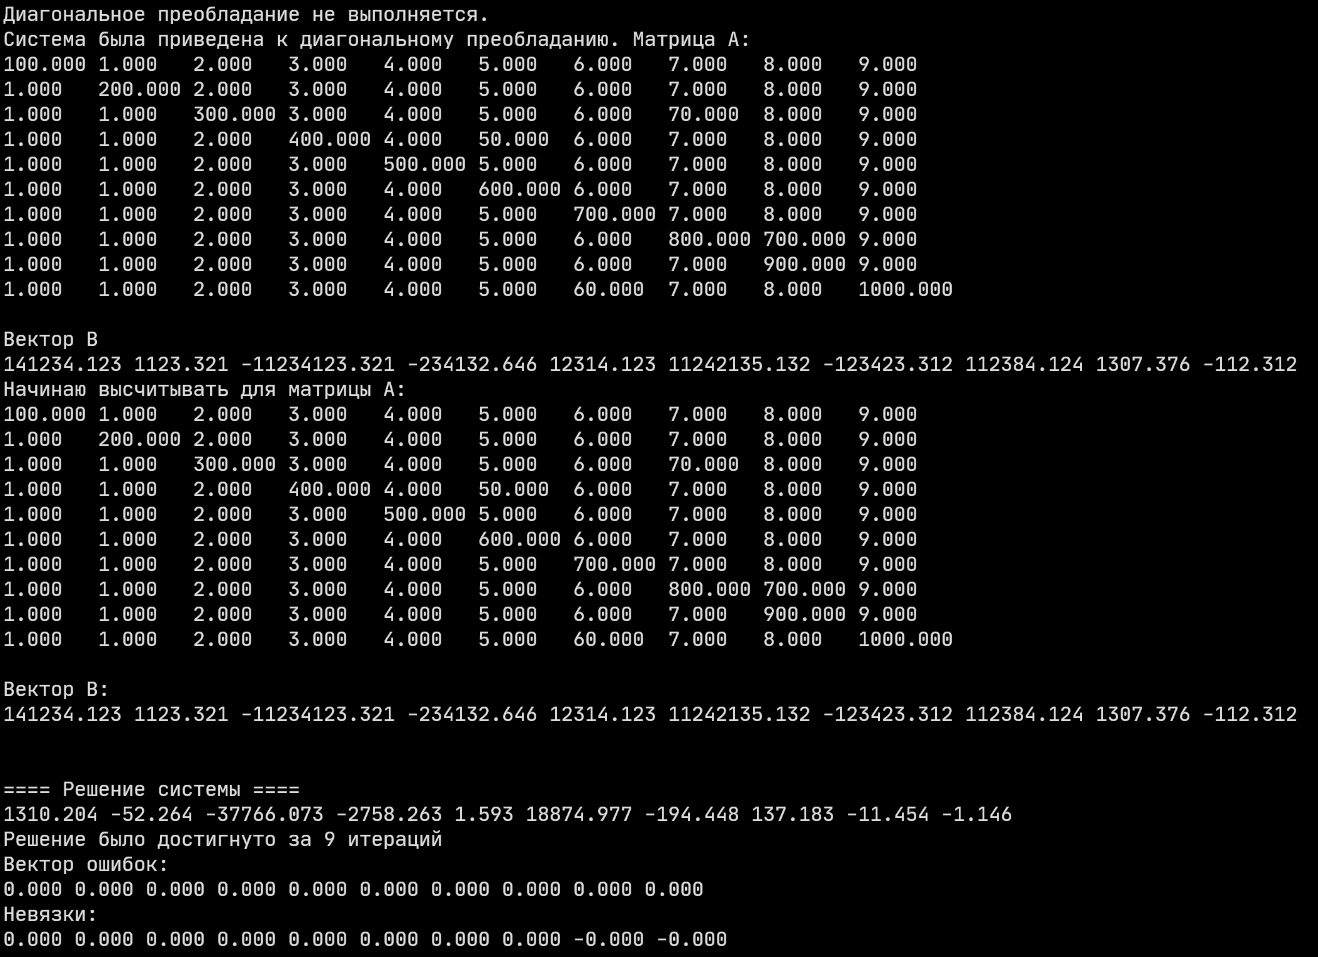
\includegraphics[width=\textwidth]{./img/test3.png}
	\caption{Работа программы для СЛАУ, заданной равенством (\ref{eq:example:3})}
	\label{fig:example:3}
\end{figure}

На рис.~\ref{fig:example:4} представлен пример работы для СЛАУ, соответствующего матрице \(A\) и вектору \(b\), заданным в (\ref{eq:example:3}),
однако последний элемент матрицы \(A_{10,10}\) был увеличен до 9000, что делает невозможным приведение матрицы к виду с диагональным доминированием.
Видно, что даже так программа находит верный в рамках погрешности ответ, однако это происходит за 20 итераций, а не за  9.

\begin{figure}[H]
	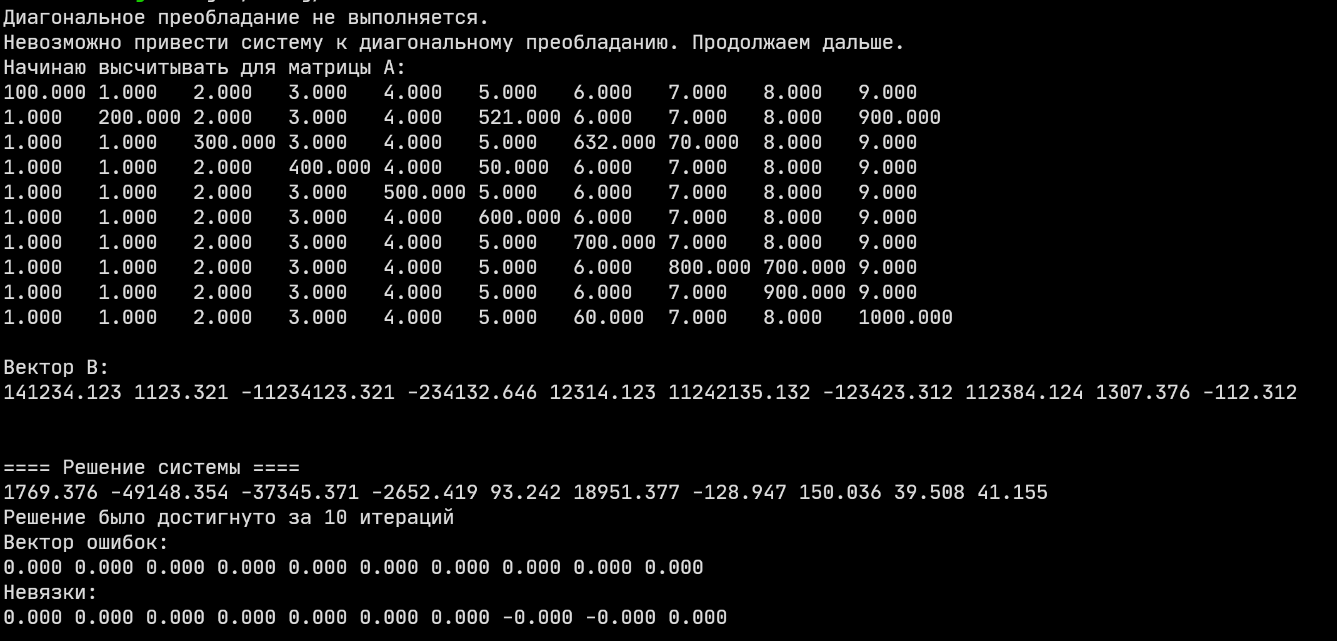
\includegraphics[width=\textwidth]{./img/test4.png}
	\caption{Работа программы для СЛАУ, заданной равенством (\ref{eq:example:3}) с увеличенным элементом \(A_{10,10}\)}
	\label{fig:example:4}
\end{figure}



\section{Вывод}
При выполнении данной лабораторной работы мною были изучены прямые методы
решения СЛАУ, а также метод простых итераций и метод Гаусса-Зейделя.
Метод Гаусса-Зейделя был реализован в обобщенной форме с помощью механизма \texttt{generics} на языке Rust.
